
%\documentclass[pre,preprint,showpacs,nofootinbib]{revtex4}
\documentclass[pre,preprint]{revtex4}
%\documentclass[article]{revtex4}
\usepackage{graphicx}
\usepackage{epsfig}
%\usepackage{dcolumn}
\usepackage{amssymb,amsmath}
\usepackage{bm}
\usepackage{pdfsync}



\newcommand{\lb}{{\langle}}
\newcommand{\rb}{{\rangle}}

\begin{document}

\title{The Diameter and Chemical Distance of Random Clusters}

\author{Don Blair}
\author{Jon Machta}

\affiliation{Department of Physics, University of Massachusetts, Amherst, MA 01003.}
\date{\today}


\begin{abstract}
 A relatively unexplored geometric property of Potts models clusters is their ``diameter'', $D$ -- the longest shortest path between any two points on the cluster. We report numerical results for the fractal dimension of the diameter, $D_{min}$ and the fractal dimension of the chemical distance, $d_{min}$, for 2D critical Potts clusters with $q=1,2,3,4,5$. We find that $D_{min} = d_{min}$ within numerical error. Test. Test2. Test3.
\end{abstract}

\maketitle 

\section{Introduction}



\begin{figure}[htp]
\centering
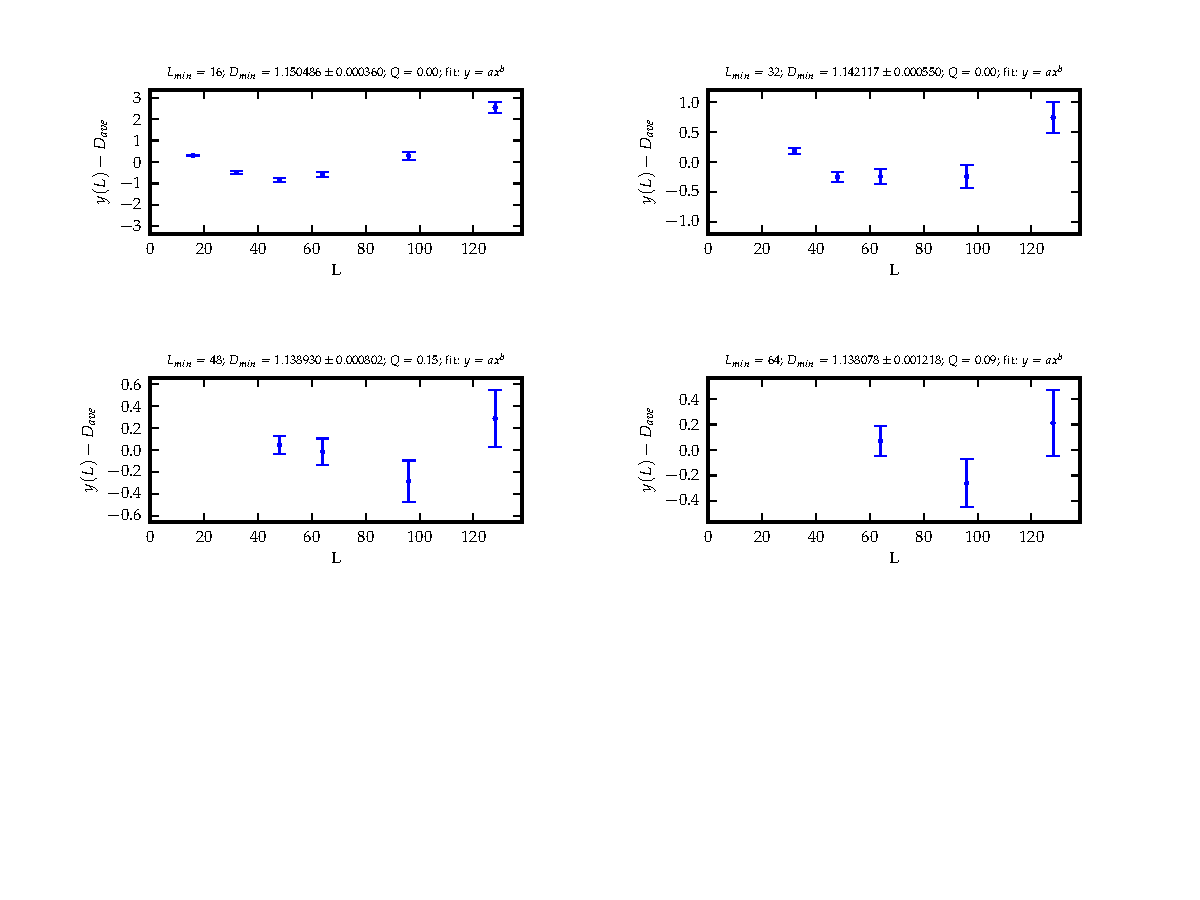
\includegraphics[width=1.1\textwidth]{figures/d_min_D2q1_42_fig}
\caption{$d_{min}$ for D=3, q=2}\label{fig:erptsqfit}
\end{figure}


\end{document}

